%\documentclass[11pt,a4paper]{report}


% The Beamer class comes with a number of default slide themes
% which change the colors and layouts of slides. Below this is a list
% of all the themes, uncomment each in turn to see what they look like.

%\usetheme{default}
%\usetheme{AnnArbor}
%\usetheme{Antibes}
%\usetheme{Bergen}
%\usetheme{Berkeley}
%\usetheme{Berlin}
%\usetheme{Boadilla}
%\usetheme{CambridgeUS}
%\usetheme{Copenhagen}
%\usetheme{Darmstadt}
%\usetheme{Dresden}
%\usetheme{Frankfurt}
%\usetheme{Goettingen}
%\usetheme{Hannover}
%\usetheme{Ilmenau}
%\usetheme{JuanLesPins}
%\usetheme{Luebeck}
%\usetheme{Madrid}
%\usetheme{Malmoe}
%\usetheme{Marburg}
%\usetheme{Montpellier}
%\usetheme{PaloAlto}
%\usetheme{Pittsburgh}
%\usetheme{Rochester}
%\usetheme{Singapore}
%\usetheme{Szeged}
%\usetheme{Warsaw}

\documentclass[10pt]{beamer}
\usepackage{float}
\usepackage[nodisplayskipstretch]{setspace}
\usepackage{pdfpages}
\usepackage{tikz}    
\usetheme{metropolis}
\usepackage{appendixnumberbeamer}
\usepackage[normalem]{ulem}
\usepackage{eurosym}
\usepackage{booktabs}
\usepackage[scale=2]{ccicons}
\usepackage[utf8]{inputenc}
\usepackage{soul}
\usepackage{mathabx}
\usepackage{graphicx}
\usepackage{pgfplots}
\usepgfplotslibrary{dateplot}
 \usepackage{relsize}
\usepackage{xspace}
\usepackage{caption}

\usepackage{graphicx}
\usepackage{graphicx}

\usepackage{hyperref}
\hypersetup{
    colorlinks=true,
    linkcolor=blue,
    filecolor=magenta,      
    urlcolor=blue,
}
 
\urlstyle{same}
\newcommand{\themename}{\textbf{\textsc{metropolis}}\xspace}


% As well as themes, the Beamer class has a number of color themes
% for any slide theme. Uncomment each of these in turn to see how it
% changes the colors of your current slide theme.

%\usecolortheme{albatross}
%\usecolortheme{beaver}
%\usecolortheme{beetle}
%\usecolortheme{crane}
%\usecolortheme{dolphin}
%\usecolortheme{dove}
%\usecolortheme{fly}
%\usecolortheme{lily}
%\usecolortheme{orchid}
%\usecolortheme{rose}
%\usecolortheme{seagull}
%\usecolortheme{seahorse}
%\usecolortheme{whale}
%\usecolortheme{wolverine}

%\setbeamertemplate{footline} % To remove the footer line in all slides uncomment this line
%\setbeamertemplate{footline}[page number] % To replace the footer line in all slides with a simple slide count uncomment this line

%\setbeamertemplate{navigation symbols}{} % To remove the navigation symbols from the bottom of all slides uncomment this line


\usepackage[utf8]{inputenc}
\usepackage{graphicx}

\usepackage{amsmath,amsthm,amssymb,latexsym,amsfonts}


\setlength{\parindent}{15pt}
\usepackage{subfig}
\usepackage{hyperref}
\usepackage{graphicx} % Allows including images
\usepackage{booktabs} % Allows the use of \toprule, \midrule and \bottomrule in tables

\usepackage{bm}

%\title{Probar que un predicado es primitivo recursivo sin marearse}
%\author{Guillermo Mosse}


%TODO todo el tiempo preguntar si hay preguntas!


\begin{document}
%TODO cambiar rojo y azul por colores que tenga marcador. No, cnseguir uno azul para pizarron

% Llego y divido el pizarrón en 2
% Hola, qué tal? Elegí contar el ejercicio de la materia Lógica y Computabilidad, que pide probar que cierto predicado es primitivo recursivo. Voy a presentar el ejercicio, su contexto, su resolución, y al final voy a dejar un par de enunciados parecidos para mis...alumnos imaginarios.

\title{Prueba de oposición 2017: Probar que cierto predicado es primitivo recursivo}
\subtitle{\small{(Sin marearse)}}
% \date{\today}
\date{}
\author{Guillermo Mosse}

\maketitle


\begin{frame}{Contexto}
\begin{itemize}

	
	% Este es el ejercicio 6 de la práctica 2; los chicos vienen trabajando con las funciones p.r. desde la práctica 1 así que voy a asumir que ya las conoce un poco y voy a usar resultados conocidos, probados en esa práctica o en la teórica; la práctica 2 es sobre funciones S-computables pero mezcla conceptos de funciones primitivas recursivas, como el ejercicio que voy a dar. Es un buen problema para resolver en clase porque hacer este tipo de ejercicios sin marearse, y de manera concisa y completa tiene sus dificultades, de las que voy a hablar en un ratito.
	% Además, es un tipo de ejercicio que suelen tomar en un parcial (a mí me tomaron uno parecido en su momento). Más aun porque relaciona el lenguaje S con las funciones p.r., lo cuál lo hace un ejercicio bien completo.

	\item Ejercicio 6 de la práctica 2.
	\item Los chicos ya conocen bastante a las funciones primitivas recursivas por la práctica 1.
	\item Hacer este tipo de ejercicios en forma concisa y completa tiene sus dificultades.
	\item Suele ser un tipo de ejercicio que se toma en un parcial.
\end{itemize}
\end{frame}    


\begin{frame}{Enunciado}

\bigskip

%Es un típico ejercicio que define algo nuevo en su mismo enunciado y luego pide, inmediatamente, trabajar con eso.

%El ejercicio dice lo siguiente: Un programa P en el lenguaje S con instrucciones I_1 a I_n se dice optimista si para todas sus instrucciones se tiene que si la instrucción es de la forma 'IF V \neq 0 GOTO L' (donde V se sobreentiende que es una variable cualquiera, y L es una etiqueta) entonces la etiqueta L no aparece antes en el programa. Una forma de pensar la definición es que el programa P nunca vuelve para atrás.

Ejercicio: Un programa $P$ en el lenguaje $S$ con instrucciones $I_1,...,I_n$ se dice optimista si $\forall\ i = 1,...,n$, si $I_i$ es la instrucción $'IF\ V \neq 0$ GOTO $L'$ entonces $L$ no aparece como etiqueta de ninguna instrucción $I_j$ con $j \leq i$.\\



% 0:53

%Dada esta definición, se pide probar que el predicado r(x) es primitivo recursivo, donde r(x) devuelve 1 si el programa de número x es optimista, y 0 si no: 
Demostrar que el siguiente predicado es primitivo recursivo:


$$r(x) = \left\{
    \begin{array}{c l}
     1    & \text{si el programa cuyo número es x es optimista}\\
	 0    & \text{caso contrario}
     
    \end{array}
    \right.
    $$

\end{frame}


%Ahora sí, pasemos a la resolución del ejercicio
\begin{frame}
\frametitle{Entendamos el enunciado}

Queremos ver que el predicado $r(x)$ es primitivo recursivo.

¿Cómo se prueba algo así? \pause

Recuerdo: una función es primitiva recursiva (p.r.) si se puede obtener a partir de las funciones iniciales por un número finito de aplicaciones de composición y recursión primitiva. \pause%Bibliografía slide 27

% ¿Cómo probamos que r(x) es p.r.?
% Bueno, sabemos que una función es p.r. si se puede obtener de las iniciales con composición y recursión primitiva,
% ...y a las iniciales ya las conocemos bastante...
% Pero si no usamos más tecnología vamos a estar mil años. ¿Qué otras herramientas tenemos? ¿Qué conocemos de las funciones p.r. que les parece que va a ser útil para la resolución del ejercicio?
% [Cambiando el tono para mostrar que le estoy hablando al jurado] Si estuviéramos en una clase de verdad esperaría, lo charlaría con los alumnos y anotaría en el pizarrón lo que dicen, pero como esta es la prueba de oposición voy a responderme yo

¿Qué herramientas tenemos a nuestra disposición?: \pause

% Muy bien carlitos, los operadores lógicos
% Bien, josefina! Todas las operaciones básicas
% No, Ignacio. La función halt no es p.r...

% [CHARLA]
%A mí se me ocurrieron estas:

\begin{itemize}
	\item El conjunto de predicados p.r. es cerrado por operadores lógicos ($\neg, \lor, \land$) %[Hacer en el pizarrón] donde cerrada significa que si \alpha y \beta son predicados funciones p.r. entonces \alpha \lor \beta también, por ejemplo
	\item El conjunto de funciones p.r. es cerrado por definición por casos %[Hacer en el pizarrón] Muestro un caso particular en una variable que es el que vamos a usar, pero vale algo mucho más general. Si g1(x),g2(x),h(x) son p.r. entonces f también
	\item Y por cuantificadores y minimizadores acotados % tal vez esto lo puedo escribir en el pizarrón
	\item También puedo usar codificación y decodificación de pares y secuencias, y longitud de secuencias
	\item Operaciones básicas (¡ojo! la resta no está, hay que usar resta con punto)
	\item Los operadores $\leq,\geq,=,\neq$, etc
	%Todas estas cosas las vieron en la práctica 1, o con Santi en la teórica. Algunas de estas herramientas las vamos a usar y otras no
\end{itemize}

\end{frame}


	% Como la función r(x) recibe un número de programa y devuelve algo en base a sus instrucciones, vamos a tener que recordar la codificación de los programas

\begin{frame}{¿Cómo se codificaba el número de programa?}

	%¿Cómo se hacía? Primero ordenamos a todas sus variables, que son numerables, asignándoles un número a cada una (empieza en 1)
	
	% Lo mismo para sus etiquetas
	% [PIZARRÓN] Y, X_1,Z_1, X_2, Z_2,...
	% donde las X_i son variables de entrada, la Y es la única variabl de salida y las Z_i son las variables temporales,...igual no vamos a trabajar con eso sino que nos vamos a quedar con las etiquetas

	Recuerdo: ¿cómo se codifican los programas? \\ \pause
	Ordenamos las variables, asignándole un número a cada una. (Este orden está fijo, no depende del programa)
	Lo mismo para sus etiquetas. \pause
	%Y, X_1, Z_1, X_2, Z_2,...
	% A,B,C,...Z,AA,AB,AC,...
	
	
	
	% Después codificamos cada instrucción de la siguiente manera, con los numeritos a,b,c y usando pares (dos veces):
	
	%El código de la instrucción I va a ser el par formado por a y el par <b,c>
	Codificamos a la instrucción $I$ con $\#(I)=<\textbf{a},<\textbf{b},\textbf{c}>>$ donde:

	% [PIZARRÓN] <d,e> es la codificación de pares, donde d y e son números naturales
	\begin{itemize}
		\item[\textbf{1}]Si $I$ tiene etiqueta $L$ entonces $\textbf{a}= \#(L)$, si no $\textbf{a}=0$.
	\item[\textbf{2}] Si la variable mencionada en $I$ es V entonces $\textbf{c} = \#(V)-1$  %siempre va a haber una variable mencionada, por eso nos podemos dar el lujo de empezar en cero. No hay un caso donde no mencionemos una variable
	\item[\textbf{3}] Si la instrucción $I$ es:
	\begin{itemize}
		\item[\textbf{3.1}] $V \leftarrow V$ entonces $\textbf{b}=0$
		\item[\textbf{3.2}] $V \leftarrow V+1$ entonces $\textbf{b}=1$
		\item[\textbf{3.3}] $V \leftarrow V-1$ entonces $\textbf{b}=2$
		\item[\textbf{3.4}] $IF\ V \neq 0\ GOTO\ L'$  entonces $\textbf{b}=\#(L')+2$  %Y si es el GOTO no ponemos b=3 sino que guardamos el número de la etiqueta del GOTO +2, para separarlo de los otros casos. Lo que va a decir b es qué tipo de instrucción es (cuál de los 4 tipos que conocemos)
	\end{itemize}
	\end{itemize}
	
	%[PIZARRÓN] escribo <a,<b,c>> con flechas indicando que a es "etiqueta", b es "tipo de instrucción", y c es "variable mencionada".
	% Pregunta: si tengo d = #(I) un número de instrucción, cómo accedo a su etiqueta? Haciendo "left", o sea, l(d)
	% Y si quiero acceder a c, tengo que hacer primero left y después right, o sea, l(r(d))
		
		%Y, finalmente, si P es un programa con instrucciones I_1 a I_n, como en el enunciado, primero codificamos sus instrucciones y su código de programa va a ser la secuencia formada por esos números, menos 1, así empieza en cero.
		
		
		Si P es un programa con instrucciones $I_1,...I_n$, su codificación va a ser $\#(P)=[\#(I_1),...,\#(I_n)]-1$ % para que empiece en cero

		% Lo importante es que esta codificación, al usar pares y secuencias, es p.r. y esto permite, dado un número de programa x, "navegar" por el código del programa de manera p.r.
		
		% No importa realmente cómo están implementadas la codificación y decodificación de pares y secuencias, abstraigámonos de todo eso.

\end{frame}


%4:30


% 6:00

\begin{frame}{Empecemos}

% La idea va a ser partir el predicado $r(x)$ en trozos más manejables, probar que estos trozos se pueden expresar de manera p.r. y después unir todo

La idea del ejercicio va a ser partir al predicado $r(x)$ en funciones que sabemos que son p.r. usando que la clase de funciones p.r. es cerrada por ciertos esquemas.\\ %Ejemplo: operadores lógicos


Quiero expresar el siguiente predicado de manera p.r.: dado un programa con número de programa x,

$$r(x) = \left\{
    \begin{array}{c l}
     1    & \text{si el programa cuyo número es x es optimista}\\
	 0    & \text{caso contrario}
     
    \end{array}
    \right.
    $$

\end{frame}


\begin{frame}{Empecemos en lenguaje (medio) coloquial}


% Digamos qué significa que un programa es optimista en lenguaje semi coloquial

Un programa con número $x$ es optimista sii:\bigskip

 $\forall i \leq n$,\\
  $[Si\ I_i\ "es"\ 'IF\ V \neq 0\ GOTO\ L' \Rightarrow\ \forall j \leq i,\ I_j\text{ no tiene la etiqueta L}]$,

 donde n es la cantidad de líneas del programa x.

% [LO COPIO EN EL PIZARRÓN +40 segundos, y voy borrando]

\end{frame}

%5:00

\begin{frame}{Vamos transformando la expresión...}

Un programa con número $x$ es optimista sii:\bigskip

 $\forall i \leq \bm{\mid x+1\mid}$,\\
 $[Si\ I_i\ "es"\ 'IF\ V \neq 0\ GOTO\ L' \Rightarrow\ \forall j \leq i,\ I_j\text{ no tiene la etiqueta L}]$
\end{frame}

\begin{frame}{Partámosla en trozos más manejables}

Un programa con número $x$ es optimista sii:\bigskip

 $\forall i \leq |x+1|$,\\
 $[$\color{red}$Si\ I_i\ "es"\ 'IF\ V \neq 0\ GOTO\ L'$\color{black}$ \Rightarrow\ $\color{blue}$\forall\ j \leq i,\ I_j\text{ no tiene la etiqueta L}]$\color{black}
 
 
 %Si pasa el predicado rojo, entonces tiene que pasar el predicado azul
\end{frame}


\begin{frame}{Primera parte}
	\color{red}$I_i\ "es"\ 'IF\ V \neq 0\ GOTO\ L'$\color{black}: \bigskip
	
	El número de programa es x. Expresemos este predicado de manera p.r.:
	
	$$p(i,x) = \left\{
    \begin{array}{c l}
     1    & si\ I_i\ "es"\ 'IF\ V \neq 0\ GOTO\ L' \\
	 0    & \text{caso contrario}
     
    \end{array}
    \right.
    $$
\end{frame}

\begin{frame}{Primera parte}
	\color{red}$I_i\ "es" 'IF\ V \neq 0\ GOTO\ L'$\color{black}: \bigskip
	
	El número de programa es x. Expresemos este predicado de manera p.r.:
	%Podemos escribir la instrucción I_i así:
	$$p(i,x) = \left\{
    \begin{array}{c l}
     1    & si\ \bm{(x+1)[i]}\ "es"\ 'IF\ V \neq 0\ GOTO\ L' \\
	 0    & \text{caso contrario}
     
    \end{array}
    \right.
    $$ \bigskip
    
\end{frame}

\begin{frame}{Primera parte}
	\color{red}$I_i\ "es"\ 'IF\ V \neq 0\ GOTO\ L'$\color{black}: \bigskip

    Recordemos que una instrucción es de la pinta $<a,<b,c>>$, donde $a$ tiene información de la etiqueta, $b$ del tipo de instrucción, y $c$ de la variable mencionada.
    
    Luego queremos que, si $I_i = <a,<b,c>>$, entonces $b\geq 3$. Queda:
    %Podemos cambiar el "es" por observadores de secuencias...
    $$p(i,x) = \left\{
    \begin{array}{c l}
     1    & si\ \bm{l(r((x+1)[i]))\geq 3}) \\
	 0    & \text{caso contrario}
     
    \end{array}
    \right.
    $$
 

\end{frame}


\begin{frame}{Segunda parte}

	% Si Emi me llega a decir algo: ¡Muy bien Emi! Es una sutileza que después pensaba contar cómo se arregla
	\color{blue}$\forall\ j\ \leq\ i, I_j\text{ no tiene la etiqueta L}$\color{black}: \pause
	
	
	$$n(i, j, x) = \left\{
    \begin{array}{c l}
     1    & si\ \forall\ j\ \leq\ i, (x+1)[j]\ \text{ no tiene la etiqueta L} \\
	 0    & \text{caso contrario}     
    \end{array}
    \right.
    $$ \bigskip
\end{frame}


\begin{frame}{Segunda parte}


	\color{blue}$\forall\ j\ \leq\ i, I_j\text{ no tiene la etiqueta L}$\color{black}: 
	
	%Pongamos de qué depende este predicado por completitud, pero es anecdótico y no va a hacer realmente falta
	$$n(x,i,j) = \left\{
    \begin{array}{c l}
     1    & si\ \forall\ j\ \leq\ i, \bm{[l((x+1)[j]) \neq l(r((x+1)[i])) \dotdiv 2]}\\
	 0    & \text{caso contrario}     
    \end{array}
    \right.
    $$ \bigskip \pause
    
    porque si $I_i$ es un GOTO, $l(r((x+1)[i]))-2$ es la etiqueta $L$, \color{red}{y, OJO, la resta con punto es p.r., la resta no.}
\end{frame}


\begin{frame}{Todo}
	Unamos todo. Queda: \\
	
	\scriptsize
	$$r(x) = \left\{
    \begin{array}{c l}
     1    & si\ \forall i \leq (|x+1|)$,[\color{red}$(l(r((x+1)[i]) \geq 3)$\color{black}$\Rightarrow$\color{blue}$(\forall j \leq i\ ([l((x+1)[j]) \neq l(r((x+1)[i])) \dotdiv 2)$\color{black}$]\\
	 0    & \text{caso contrario}     
    \end{array}
    \right.
    $$ \pause
    
    \normalsize
        
    
    Tenemos que el predicado $p \Rightarrow n$ es equivalente a $n \lor \neg p$ \pause
    
	% Suele ser un ejercicio de la primer práctica de Álgebra 1; y se prueba comparando las tablas de verdad de ambas expresiones.	
	
    Luego puedo expresar r(x) así: \pause
    
    
	\scriptsize
	    
    $$r(x) = \left\{
    \begin{array}{c l}
     1    & si\ \forall i \leq (|x+1|)$,[\color{blue}$(\forall j \leq i\ (l(x+1)[j] \neq l(r((x+1)[i])) \dotdiv 2))$\color{black}$ \lor\ \neg\ $\color{red}$(l(r((x+1)[i]) \geq 3)$\color{black}]$\\
	 0    & \text{caso contrario}     
    \end{array}
    \right.
    $$, \pause
    
    \normalsize
    
    que es p.r. por estar definido por casos por funciones p.r., donde la segunda función es la constante cero y la primera está formada por $\neg, \lor$, dos cuantificadores acotados, la longitud de una secuencia, observadores de secuencias, el predicado $\leq$ y las operaciones elementales suma y resta con punto, que sabemos que son p.r.
\end{frame}

\iffalse
\begin{frame}{Sutileza}

\scriptsize
 $$r(x) = \left\{
    \begin{array}{c l}
     1    & si\ \forall i \leq (|x+1|)$, [\color{blue}$(\forall j \leq i\  (l(x+1)[j] = (x+1)[i]-2))$\color{black}$ \lor\ \neg\ $\color{red}$(l(r((x+1)[i]) \geq 3)$\color{black}$]\\
	 0    & \text{caso contrario}     
    \end{array}
    \right.
    $$% \pause
    
\normalsize

%Si para algún $i$ la instrucción $I_i$ no es un GOTO, $(l(r((x+1)[i]) - 2$ daría negativo. Esto se arregla cambiando $(l(r((x+1)[i]))) - 2$ por $(x+1)[i] \overset{\textbf{.}}{-} 2$ (la resta con punto definida en la pr 1). No importa cuánto da esto si $I_i$ no es un GOTO porque no se cumple el antecedente, solo importa que quede bien definido. Queda:

%\scriptsize
% $$r(x) = \left\{
%    \begin{array}{c l}
%     1    & si\ \forall i \leq (|x+1|)$, [\color{blue}$(\forall j \leq i\  (l(x+1)[j] = (l(r((x+1)[i])\overset{\textbf{.}}{-} 2))$\color{black}$ \lor\ \neg\ $\color{red}$(l(r((x+1)[i]))) \geq 3)$\color{black}$]\\
%	 0    & \text{caso contrario}     
%    \end{array}
%    \right.
%    $$



\end{frame}
\fi


\begin{frame}{Es parecido:} %Ya que les quemé un ejercicio de la práctica...

	Ejercicio de parcial: Decimos que un programa es "vueltero" si en algún lugar de su código aparece la siguiente secuencia de instrucciones:
	
	$$V\leftarrow V+1$$
	$$[L]\ IF\ V \neq 0\ GOTO\ L$$
	
	para alguna variable $V$ cualquiera y alguna etiqueta $L$ que no aparece en las líneas anteriores del código del programa.
	Demostrar que el conjunto $\{x\ |\ \text{x es el número de un programa "vueltero"}\}$ es p.r.

\end{frame}



\begin{frame}
\frametitle{¿Preguntas?}

\textbf{¡Gracias por escuchar!}

\textbf{¿Alguna pregunta?}

%\begin{figure}
  %\centering
 %   \reflectbox{%
  %    
\includegraphics[scale=0.05]{anillo.png}}
  %\captionsetup{labelformat=empty}
  %\caption{1 ring}
%\end{figure}

%\hspace{\fill}

%\begin{figure}
 % \centering
 %   \reflectbox{%
  %    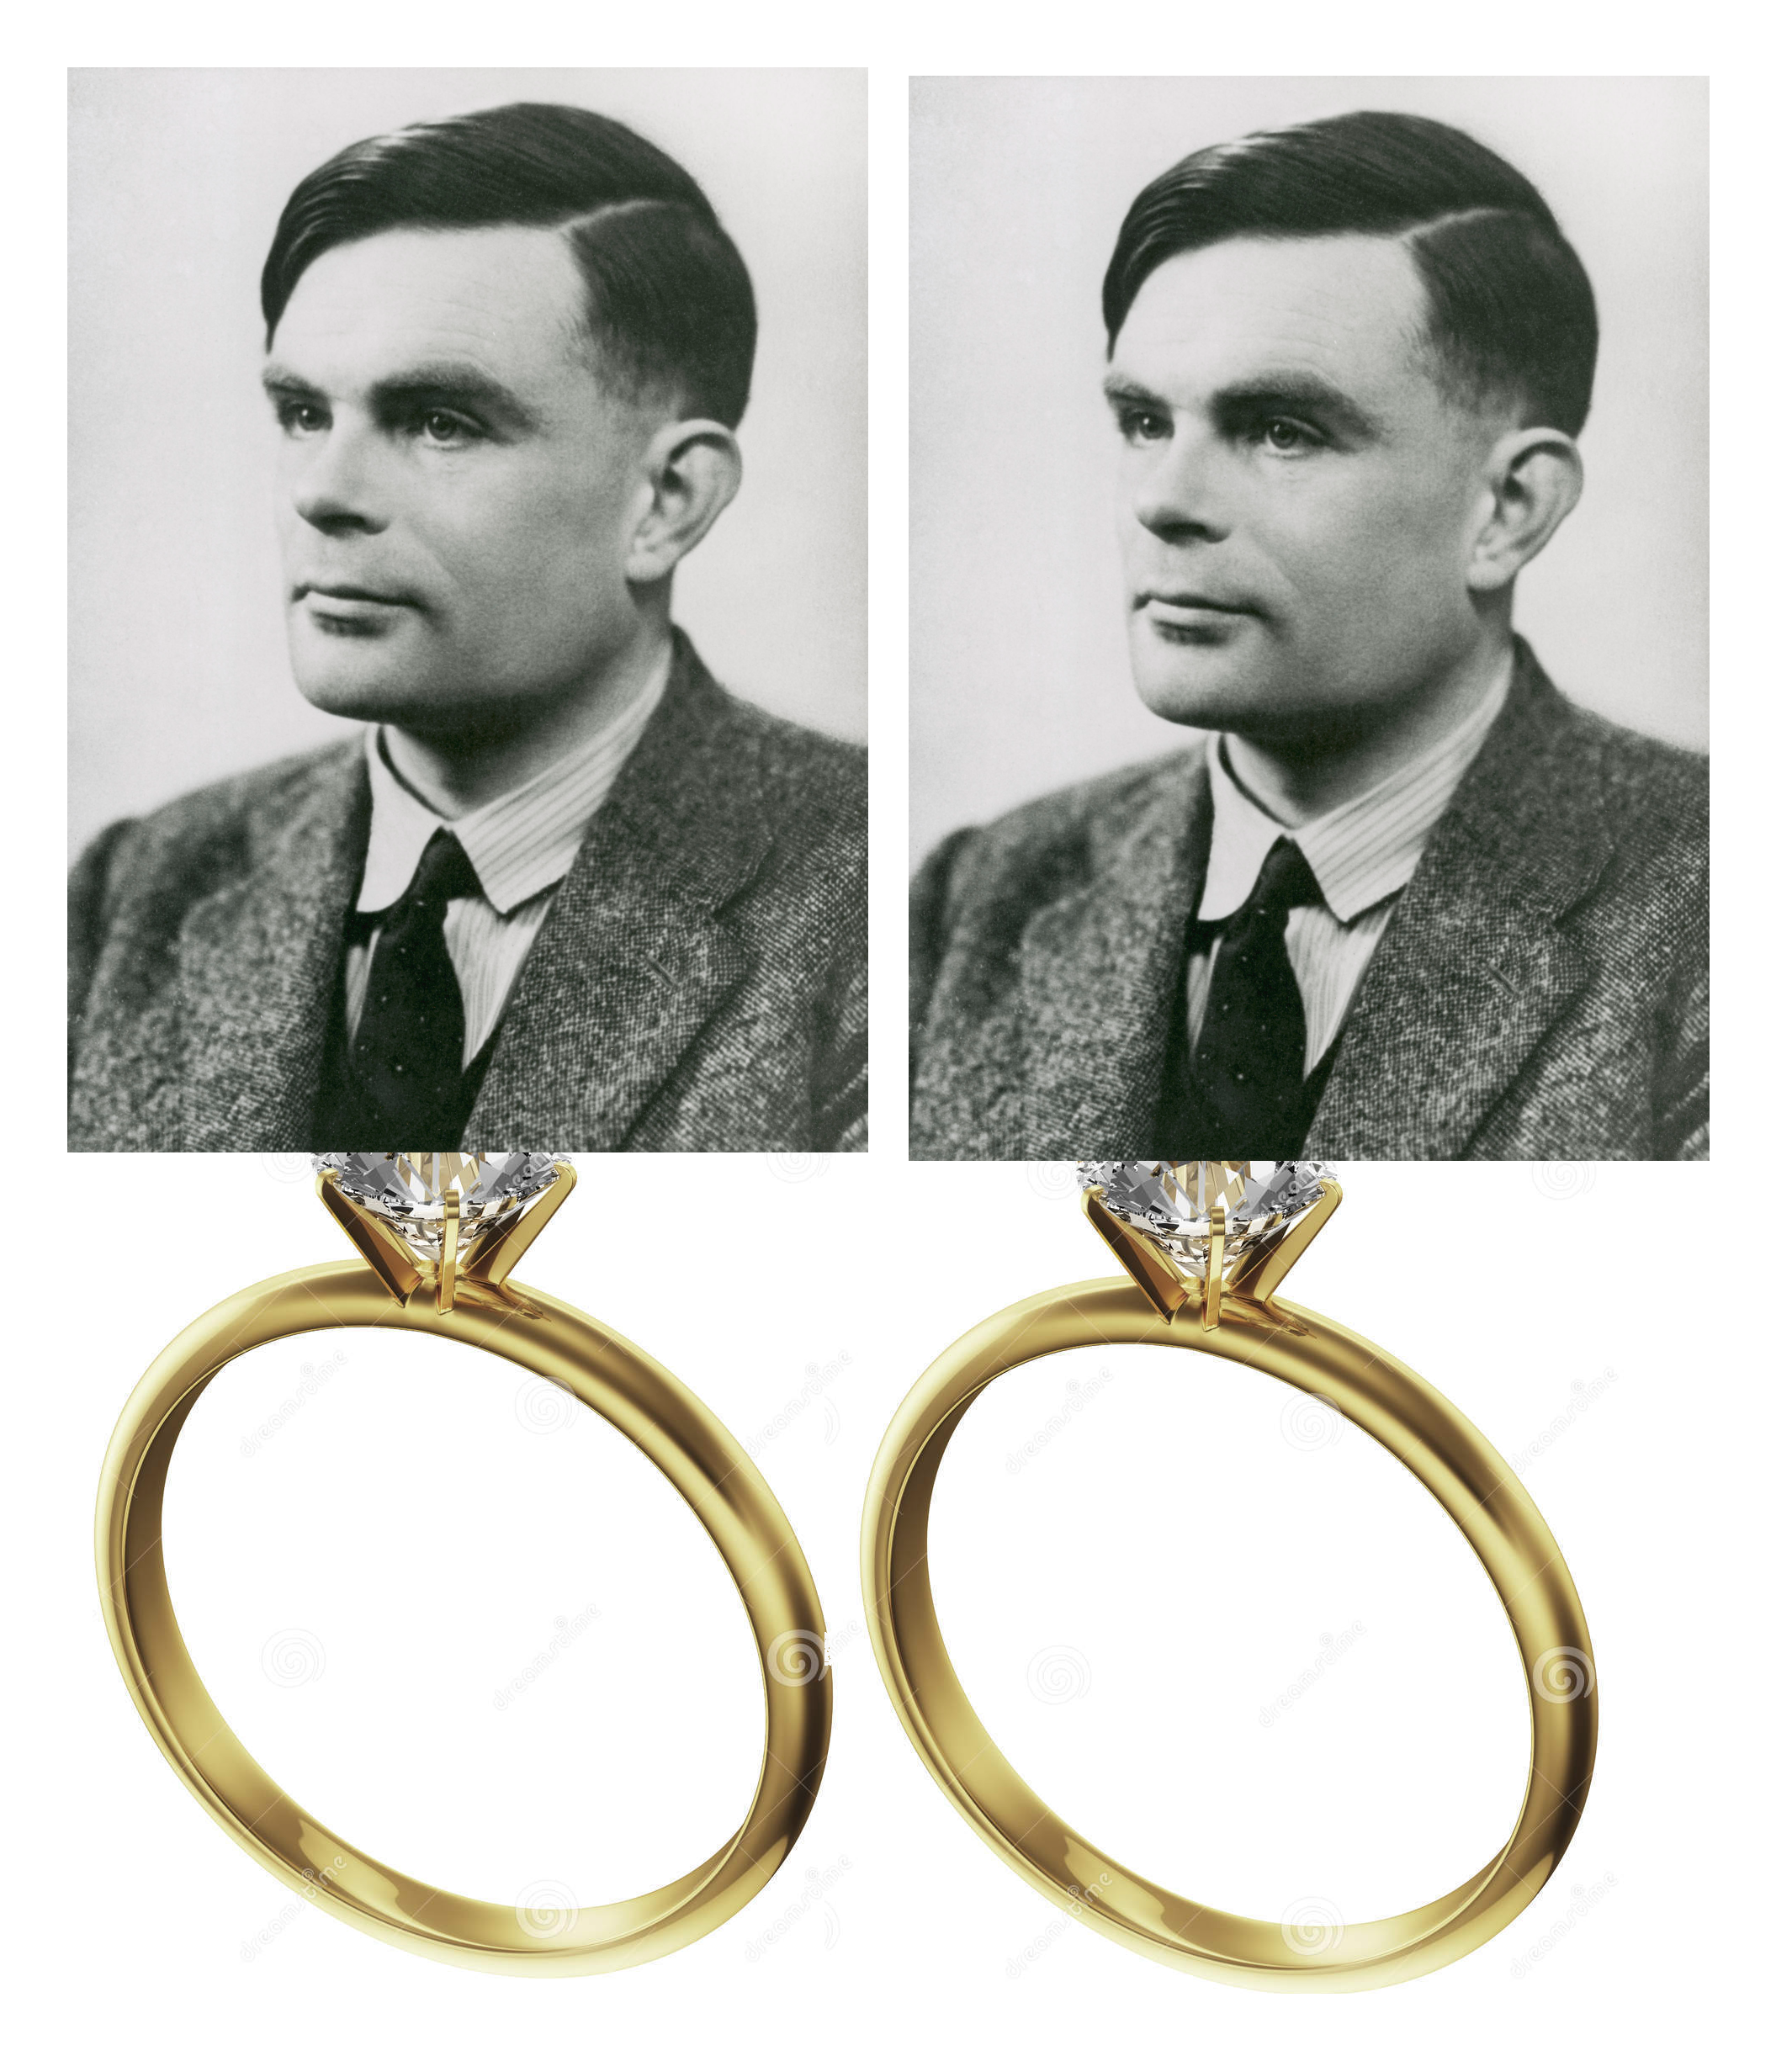
\includegraphics[scale=0.05]{anillo2.png}}
  %\captionsetup{labelformat=empty}
  %\caption{2 rings}
%\end{figure}

\begin{figure}[!tbp]
  \centering
    \captionsetup{labelformat=empty}
  \subfloat[1 ring]{
\includegraphics[scale=0.05,width=0.4\textwidth]{anillo.png}\label{fig:f1}}
  \hfill
    \captionsetup{labelformat=empty}
  \subfloat[Tu-rings]{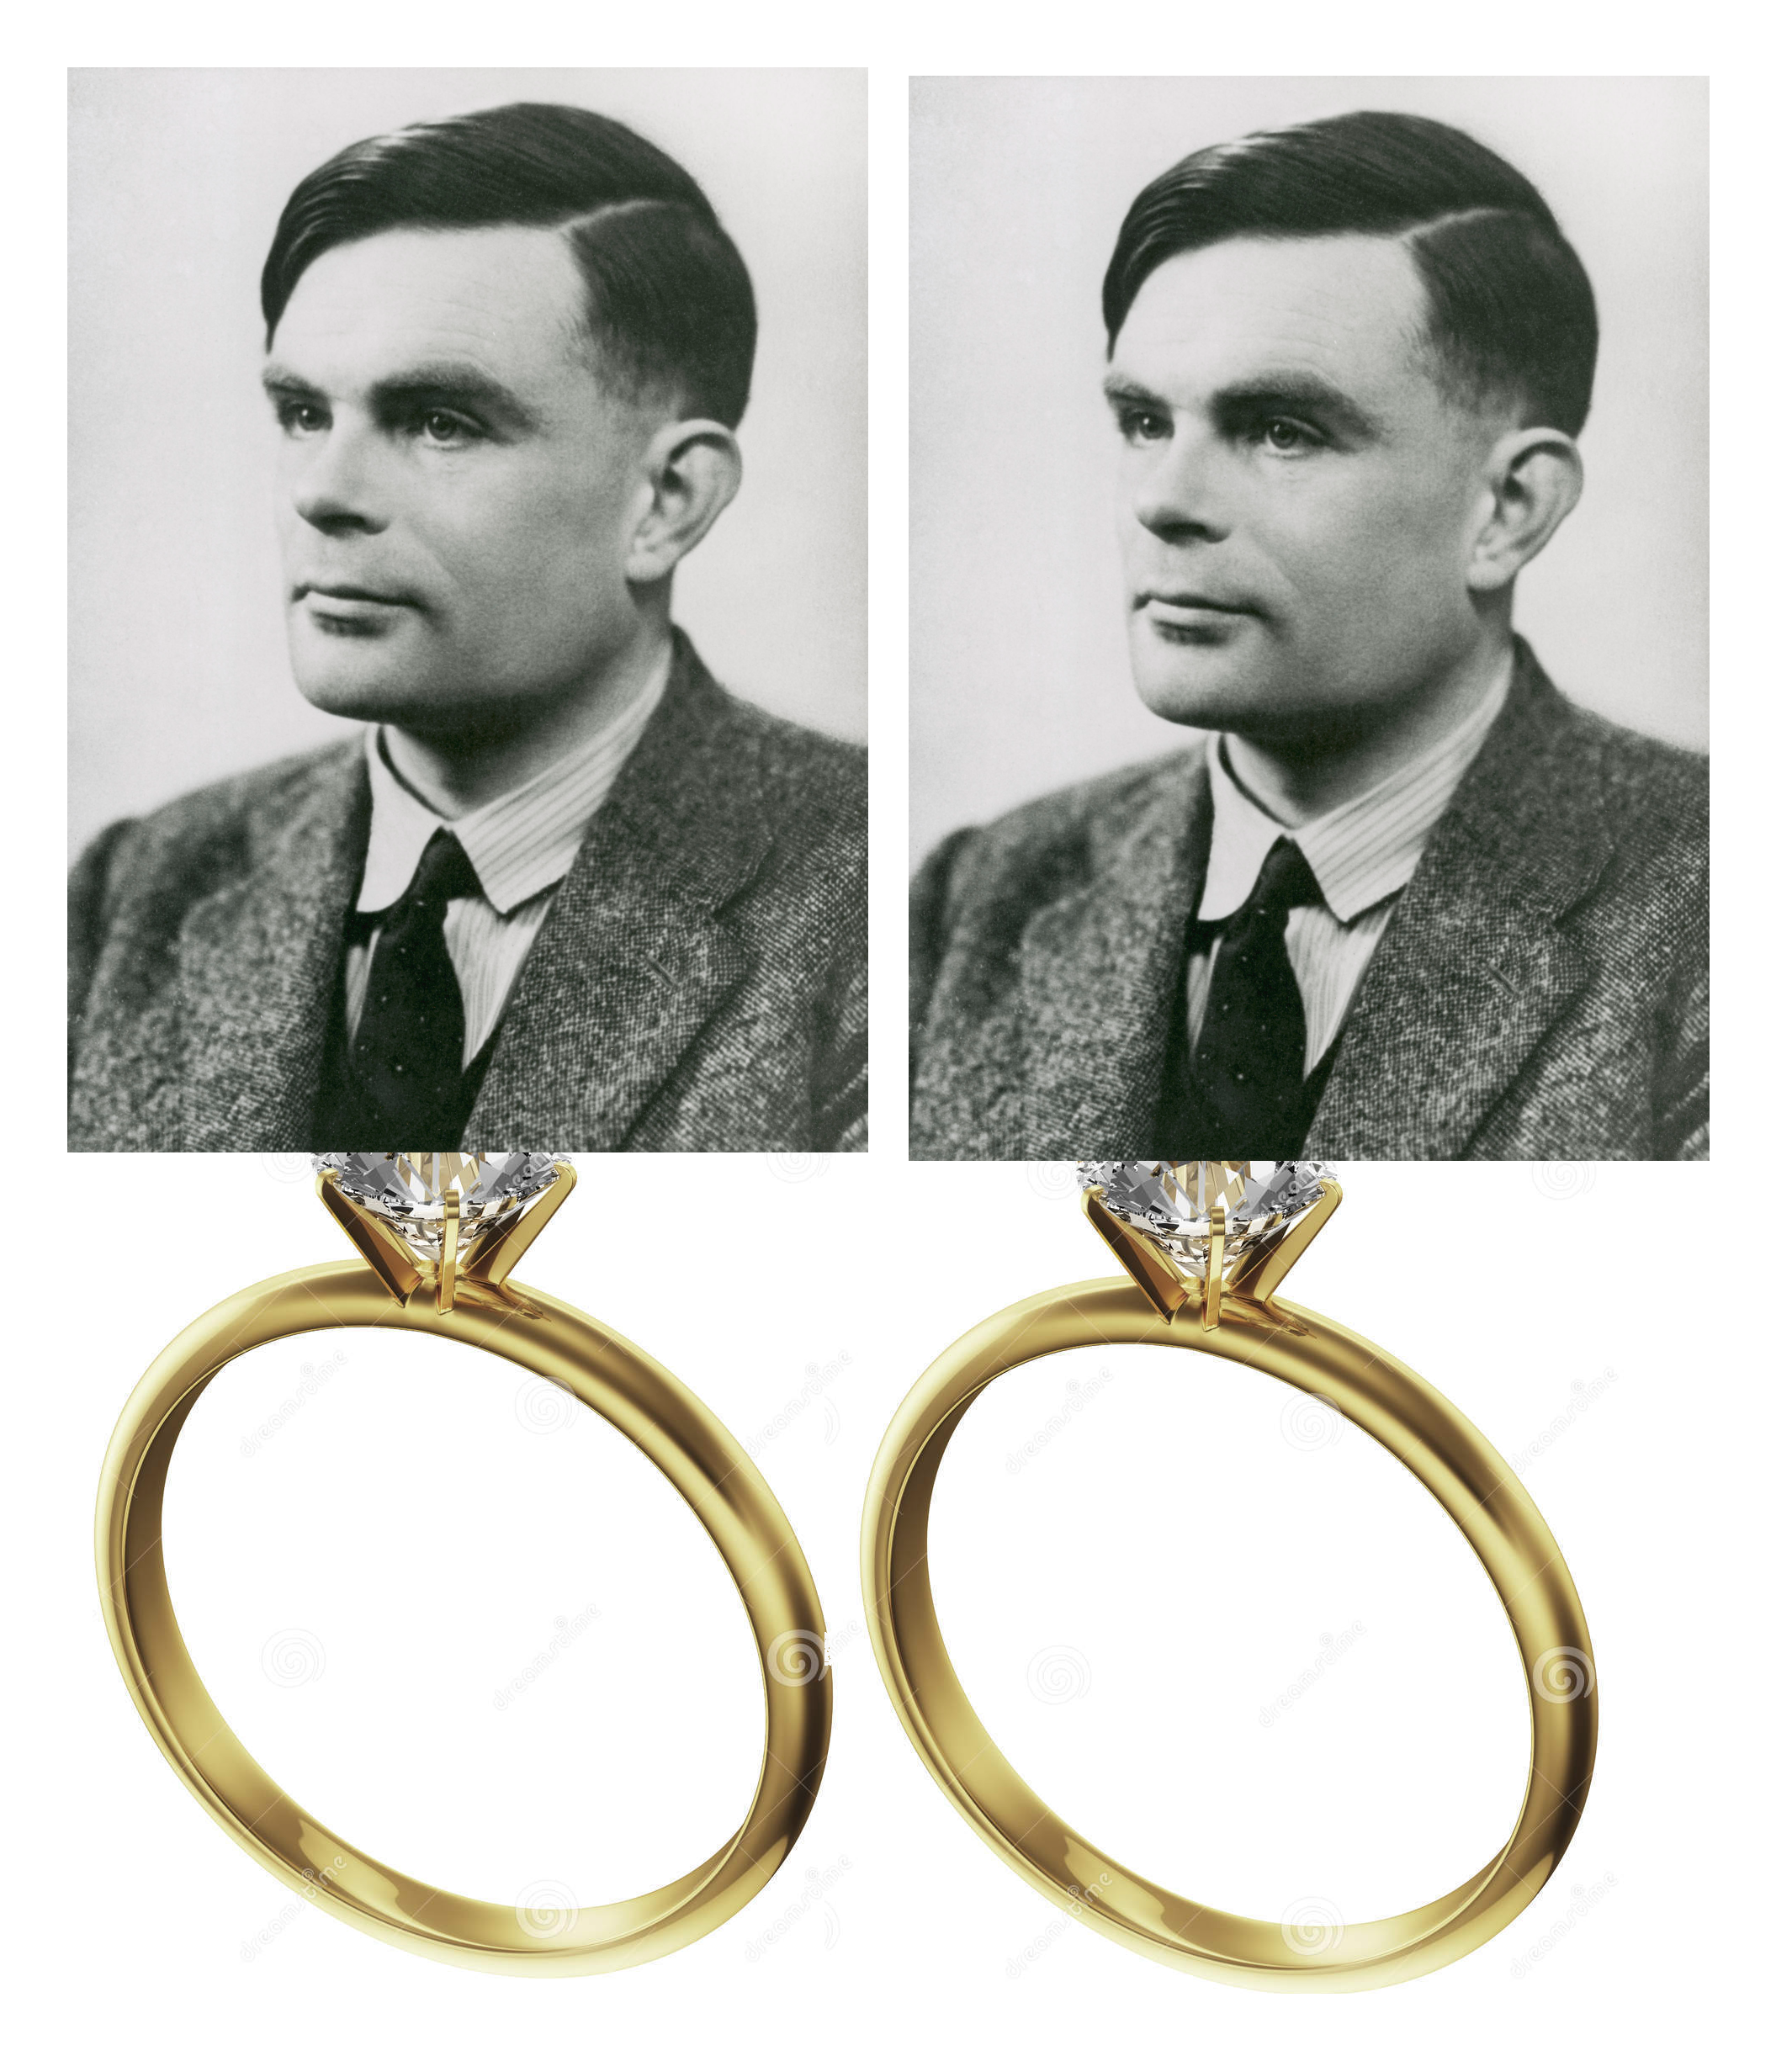
\includegraphics[scale=0.05,width=0.4\textwidth]{anillo2.png}\label{fig:f2}}
\end{figure}

\end{frame}


%Si alguien se quedó con ganas de ver cómo se trabajaba con pares y secuencias y por qué las funciones quedaban p.r., se los dejo copiado en este mini apéndice:

\setstretch{0.4}
\begin{frame}{Mini apéndice}
	$$x \dotdiv y = \left\{
    \begin{array}{c l}
     x-y    &si\ y\leq x \\
	 0    &si\ y > x     
    \end{array}
    \right.
    $$
    
    $$\textbf{Codif de pares: }<x,y> = 2^x (2 \cdot y +1) \dotdiv 1$$
    
    $$\textbf{Decodif (izq) de pares: }l(z) = min_{x\leq z} ((\exists y)_{\leq z} z = <x,y>)$$
    
    $$\textbf{Decodif (der) de pares: }r(z) = min_{y\leq z} ((\exists x)_{\leq z} z = <x,y>)$$
    
    $$\textbf{Codif de secuencias: }[a_1,...,a_n] = \prod_{i=1}^n {p_i}^{a_i}\text{, donde }p_i\text{ es el i-ésimo primo.}$$
    
	    $$\textbf{Decodif de secuencias: }x[i]=min_{t\leq x}(\neg{p_i}^{t+1} | x)$$

$$\textbf{Tamaño de secuencias: }|x| = min_{i\leq x} (x[i] \neq 0 \land (\forall j)_{\leq x} (j\leq i \lor x[j] = 0))$$
\end{frame}

% Y por último, les dejo la bibliografía que usé para armar el ejercicio
\begin{frame}
\frametitle{Bibliografía}

\begin{itemize}
	\item Teóricas de LyC, diapositivas 39-51, 75-78
	\item Práctica 1 LyC
	\item Parcial de Computabilidad del 2do cuatrimestre del 2015 \href{http://www.cubawiki.com.ar/images/1/13/LogicaYcomputabilidad_1p_2c2015.pdf}{(Link)}
	
\end{itemize}

\end{frame}


%El ¡Recordemos! lo hago en el pizarrón. Qué recuerdo?
%Qué es una valuación, que está definida sobre las variables proposicionales y %que se extiende a las otras cosas,
%y que lo de arriba es que para toda valuación sea válida.


%
%\begin{frame}
%
%\begin{itemize}
%\item Hola \alt<1>{bla}{ble}
%\item Hola \alt<2>{bla}{ble}
%
%\end{itemize}
%
%\end{frame}



%Ejercicio (tarea): Sea L un lenguaje de primer orden con igualdad y un símbolo de predicado binario R. Decidir si es posible expresar en primer orden la propiedad que afirma que existe k $\in$ N tal que todo elemento se relaciona a lo sumo con k elementos distintos.


\end{document}

%
%\tableofcontents
%\part{Addition and Subtraction}
%\chapter{Addition} \chaptercontent
%\chapter{Subtraction} \chaptercontent
%\part{Multiplication and Division}
%\chapter{Multiplication} \chaptercontent
%\chapter{Division} \chaptercontent
%\end{document}